%% ****** Start of file apstemplate.tex ****** %
%%
%%
%%   This file is part of the APS files in the REVTeX 4 distribution.
%%   Version 4.1r of REVTeX, August 2010
%%
%%
%%   Copyright (c) 2001, 2009, 2010 The American Physical Society.
%%
%%   See the REVTeX 4 README file for restrictions and more information.
%%
%
% This is a template for producing manuscripts for use with REVTEX 4.0
% Copy this file to another name and then work on that file.
% That way, you always have this original template file to use.
%
% Group addresses by affiliation; use superscriptaddress for long
% author lists, or if there are many overlapping affiliations.
% For Phys. Rev. appearance, change preprint to twocolumn.
% Choose pra, prb, prc, prd, pre, prl, prstab, prstper, or rmp for journal
%  Add 'draft' option to mark overfull boxes with black boxes
%  Add 'showpacs' option to make PACS codes appear
%  Add 'showkeys' option to make keywords appear
\documentclass[aps,pra,preprint,groupedaddress]{revtex4-1}
%\documentclass[aps,prl,preprint,superscriptaddress]{revtex4-1}
%\documentclass[aps,prl,reprint,groupedaddress]{revtex4-1}

\usepackage{graphicx}
\usepackage{amsmath}

% You should use BibTeX and apsrev.bst for references
% Choosing a journal automatically selects the correct APS
% BibTeX style file (bst file), so only uncomment the line
% below if necessary.
%\bibliographystyle{apsrev4-1}

\begin{document}

% Use the \preprint command to place your local institutional report
% number in the upper righthand corner of the title page in preprint mode.
% Multiple \preprint commands are allowed.
% Use the 'preprintnumbers' class option to override journal defaults
% to display numbers if necessary
%\preprint{}

%Title of paper
\title{Phase Dependent Ionization of Rydberg Atoms in Static Fields}

% repeat the \author .. \affiliation  etc. as needed
% \email, \thanks, \homepage, \altaffiliation all apply to the current
% author. Explanatory text should go in the []'s, actual e-mail
% address or url should go in the {}'s for \email and \homepage.
% Please use the appropriate macro foreach each type of information

% \affiliation command applies to all authors since the last
% \affiliation command. The \affiliation command should follow the
% other information
% \affiliation can be followed by \email, \homepage, \thanks as well.
\author{Eric Magnuson}
\email[]{edm5gb@virginia.edu}
\author{Tom Gallagher}
%\homepage[]{Your web page}
%\thanks{}
%\altaffiliation{}
\affiliation{University of Virginia, Department of Physics}

%Collaboration name if desired (requires use of superscriptaddress
%option in \documentclass). \noaffiliation is required (may also be
%used with the \author command).
%\collaboration can be followed by \email, \homepage, \thanks as well.
%\collaboration{}
%\noaffiliation

\date{\today}

\begin{abstract}
Pump-probe schemes using high frequency pulsed light synchronous to strong field low frequency fields are a prolific tool for probing atomic, molecular and surface electron dynamics. We realize one such system in Rydberg states of Li using an 819-nm excitation laser amplutde modulated synchronously to a 15.9-GHz microwave field. We show that when the modulation is at the same frequency of the microwave field, phase dependent ionization is only observed in the presence of static fields. Our results are well described by a computational model. Analysis of this model shows the importance of multiple classical electron orbits.
\end{abstract}

% insert suggested PACS numbers in braces on next line
\pacs{}
% insert suggested keywords - APS authors don't need to do this
%\keywords{}

%\maketitle must follow title, authors, abstract, \pacs, and \keywords
\maketitle

% body of paper here - Use proper section commands
% References should be done using the \cite, \ref, and \label commands
% Put \label in argument of \section for cross-referencing
%\section{\label{}}
%\subsection{}
%\subsubsection{}

\section{\label{sec:intro}Introduction}

Attosecond-IR experiments very useful. Test understanding of ionization in strong-field + Coulomb regime. High-harmonic-generation. Attosecond streaking to use strong fields to get time-resolved electron dynamics, ultrafast chemistry, and probe internal structure of large atoms / molecules.

The techniques and principles of attosecond-IR experiments have more broad appeal. THz experiments w/ pulsed ps, fs or as lasers use similar concepts experimental principles. Past work has extended this to application in Rydberg atoms using MW fields and pulsed excitation lasers. Shown phase dependent ionization, provided tool for probing the dynamics of Rydberg electrons near the ionization limit.

We now show the effect of breaking symmetry of system by adding pulsed electric field during excitation. Comparable to symmetry arguments used in THz and Attosecond experiments.

We provide further improvements to the computational model.


\section{\label{sec:back} Background}

Qualitatively describe behavior of electrons near ionization limit in MW fields, and recent work (Alexandr). Rydberg states with long lifetimes in strong MW field. Long orbits.

Include simpleman's + coulomb model discussed in Shuman and Overstreet. Maximum energy exchange at what phase? Describe qualitatively the process this model describes: Electron leaves core exchanging energy w/ MW field. Goes on an orbit in the static field that either ionizes or doesn't. Returning to the core, the electron can exchange energy again, the process repeats. Long orbits protect bound states from returning and maybe getting ionized.

(MAYBE) show how these calculations give a $\Delta E$ vs $\phi_0$ for initially leaving the core, and a return.

Show that when probing with a amplitude modulated laser, the observations can only be at the modulation frequency.

Show that symmetry arguments limit what harmonics of the MW field the system response can include.

(MAYBE) Show that if we limit system response to what initial energy transfer happens, this limits the phase of the phase-dependent signal to particular phases ($7\pi/6$ and $\pi/6$ in static fields, ($\pi/6$ and $7\pi/6$) or ($4\pi/6$ and $11\pi/6$) in zero field.

\section{\label{sec:exp} Experimental Methods}

Note: \emph{INCLUDE LEVEL DIAGRAM}

In this experiment, Li atoms in a collimated thermal beam are optically excited to high lying Rydberg or continuum states along the path $2s \xrightarrow{\text{671 nm}} 2p \xrightarrow{\text{610 nm}} 3d \xrightarrow{\text{819 nm}} nf, \epsilon f$. These optical beams intersect at a right angle forming a rectangular 1 mm$^3$ excitation region. This region is at an anti-node of a 15.9 GHz Fabry-Perot microwave cavity. The excitation occurs in the presence of microwave fields, so that the $nf, \epsilon f$ electron exchanges energy with the field as it leaves the atomic core.

% (THIS IS ALL MENTIONED LATER) The 1 mm$^3$ region is much smaller than the extent of the microwave antinode, allowing us to consider the microwave field constant across the region. The interaction region is enclosed on top, bottom and two sides by aluminum plates. Combined with the two Fabry-Perot mirrors, this forms a 10-cm cubic enclosure. Bias voltages can be applied independently to each plate and mirror to control static fields in the interaction region.

The microwave cavity is allowed to load for 240 ns before the first laser pulse, and the microwave input is shut off 20 ns after the last laser pulse, allowing the cavity to empty. Synchronous with the MW power envelope, a static field pulse is applied to the top and bottom aluminum plates to produce a vertical static field in the interaction region. The 610-nm and 671-nm lasers are pulsed synchronously for 20 ns, after which the 819-nm laser is pulsed with a square envelope for 20 ns. One microsecond after the last laser pulse, we field ionize surviving Rydberg states within 100 GHz of the ionization limit by applying a negative voltage pulse to an aluminum plate below the interaction region. Ionized electrons are pushed into a microchannel plate (MCP) assembly which produces a voltage pulse proportional to the number of electrons detected. This pulse is integrated through a boxcar integrator and recorded.

The signal detected is normalized to the signal from the total number excited electrons. The total excitation ($S_{total}$) is measured by applying the field ionization pulse during excitation, so all Rydberg and continuum states are driven to the detector. This value is compared to the signal observed when the field ionization pulse occurs 1 $\mu$s after the final laser pulse, which only detects bound Rydberg states $S_{Ryd}$. Signals reported in this paper always show $S = S_{Ryd} / S_{total}$.

\begin{figure}
	\includegraphics[width=0.5\textwidth]{fields}
	\caption{Temporal view of the microwave field (top) phase-locked with the amplitude modulated laser intensity (bottom). The peak laser intensity occurs at the phase $\omega_0 t$ of the microwave field, and can be adjusted by an optical delay line.}
	\label{fig:AMLaser}
\end{figure}

Probing phase dependence in this experiment is achieved by synchronizing the amplitude modulation of the 819-nm laser to a microwave field in the cavity, as shown in Fig.~\ref{fig:AMLaser}. The laser field can be described by an envelope modulating a fundamental frequency:
\begin{equation}
E_{opt}(t) = E_o \sin{(\omega_o t)} \cos{(\omega(t-t_0))}
\end{equation}
The 
Using an optical delay line, the phase of the modulation envelope of the 819-nm laser can be delayed relative to phase of the microwave field. This modulation is proportional to the excitation-rate to a Rydberg or continuum state, so delaying the modulation envelope is equivalent to changing the phase $\omega t_0$ of the microwave field at which excitation occurs.

\subsection{\label{sec:dye} Dye Lasers}

We use two dye lasers at 670-nm and 610-nm to drive the $2s \rightarrow 2p$ and $2p \rightarrow 3d$ transitions, respectively. These dye lasers are pumped by a Quantronix Darwin Nd:YLF. The pump laser produces 30-W, approximately 100-ns FWHM pulses at a 1-kHz repetition rate. Using a Pockels cell (PC) and polarizing beam splitter (PBS), the rising edge of the pulse is picked off and split equally between to the 670-nm and 610-nm lasers. A second PC and PBS directs a 20-ns slice from the peak of the pump pulse to a dye amplifier for the 819-nm laser. The long trailing edge of the pump pulse is dumped.

The 670-nm dye laser uses a Littman-style cavity and LDS-698 laser dye dissolved in Ethanol as a lasing medium. The 610-nm uses a H{\"a}nch style cavity with Rhodamine-610 laser dye dissolved in Ethanol. Both lasers have an approximate FWHM of 10-GHz. To minimize unintended ionization from the $3d$ state, both lasers are attenuated to 2 $\mu J$ pulses before being directed to the vacuum chamber.

\subsection{\label{sec:ampmod} Amplitude Modulated 819 nm Laser}

\begin{figure}
	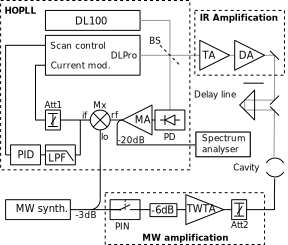
\includegraphics[width=0.5\textwidth]{beatexp}
	\caption{Schematic showing how the amplitude modulated laser is produced, locked to the microwave frequency, and how both the laser and microwave fields are delivered to the interaction region. The AM IR laser is generated by overlapping the DL-Pro and DL-100 laser beams on a beamsplitter (BS). One output is amplified and sent to the interaction region. The microwave field is generated by a synthesizer, formed into pulses by the PIN switch and amplified by the Traveling Wave Tube Amplifier (TWTA) before injection into the microwave cavity. The locking of the IR intensity envelope to the microwave field is performed by the Heterodyne Optical Phase Locked Loop (HOPPL).}
	\label{fig:pll}
\end{figure}

Fig.~\ref{fig:pll} shows how the amplitude modulated laser and microwave fields are produced and delivered to the interaction region, and how they are locked in a phase locked loop. The 819-nm laser is produced from two external-cavity diode lasers, a Toptica DL-100 and DL-Pro. The lasers are tuned such that their frequencies are separated by the microwave frequency, and the two beams are overlapped on a 50:50 beamsplitter (BS). This overlapping produces a beat-note in the laser intensity at the microwave frequency. One output from the beamsplitter is directed to a high speed photodetector that can detect the beat note and deliver the signal to the phase-locked-loop. The second output from the beamsplitter is directed through an amplification chain and to the interaction region.

The amplitude modulation of the laser is locked to the microwave frequency with a heterodyne optical phase-locked-loop (HOPLL). The locking is driven by a "fast" feedback to the current input of the DL-Pro, and a "slow" feedback to the scan input. To produce an error signal, the amplitude modulation is detected after the 50:50 beamsplitter by a fast photodiode. The DC signal is filtered out, leaving only the AC component. This is amplified and mixed with the microwave source to produce an error signal. The error signal is passed through a variable attenuator and then connected to the Current input of the Toptica DL-100. This achieves a lock between the laser ampltude modulation frequency and the microwave field that lasts for several minutes.

To achieve longer lock times on the order of hours, we use a Toptica PID-110 to drive the scan input of the DL-Pro. The "fast" current lock is primarily lost due to the lasers drifting past the range that the current input can correct. Low-frequency components of the error signal are processed through a PID and fed to the Scan input. This corrects long term drifts in the amplitude modulation frequency, leaving only high-frequency errors for the "fast" loop to correct.

The second output of the 50:50 beamsplitter produces 30 mW of aplitude modulated light. This is passed through a tapered amplifier and a dye amplifier. The Toptica Tapered Amplifier increases the continuous beam power to 800 mW. The dye amplifier is pumped by a 20-ns square pulse picked from the peak of the Nd:YLF laser pulse. We use LDS-819 dissolved in Ethanol as the amplfication medium. This produces a 20 ns long, 6 $\mu$W pulse of amplitude modulated 819-nm light.

Once locked, the AM phase at the BS is constant relative to the MW phase, and their relative phase in the interaction region depends only on the effective path length difference. To adjust the path length of the AM laser beam, after amplification the beam is passed through an optical delay before continuing to the interaction region. This optical delay consists of a retro-reflector mounted to a translation stage, able to extend the path length of the AM laser by several MW wavelengths.

\subsection{\label{cavity} Microwave Apparatus}

A Hittite HMC T-2100 synthesizer tuned to the 15.9-GHz resonance of the microwave cavity is used as our microwave source. The Hittite produces 9 dBm, and a splitter diverts half of the power to the microwave mixer to generate the error signal for the PLL. The other half of the signal is formed into 300-ns pulses by a microwave switch, and then amplified by a Hughes 8020H04F traveling-wave-tube-amplifier (TWTA). Between the TWTA and the cavity, there is a 0 to 50 dBm variable attenuator allowing us to control the intensity of the pulse incident on the microwave cavity.

The microwave cavity is a Fabry-Perot cavity composed to two brass spherical mirrors. These mirrors have a radius of curvature of 10 cm and are 10.2 cm in diameter, with an on axis separation of 7.83 cm. The 15.9 GHz resonance is the TEM$_{008}$ mode of the cavity, with a quality of 3600. We are able to determine the field inside the cavity to \emph{15\%}.

\subsection{\label{fields} Static Fields}

This experiment depends on the detection of long lived Rydberg states close to the ionization limit. To prevent these states from ionizing before detection, we must minimize the persistent static field in the interaction region. We accomplish this by surrounding the interaction region on two sides with the brass microwave cavity mirrors, and on the remaining two sides, top, and bottom with polished aluminum plates. A voltage can be applied independently to each plate or mirror, allowing us to compensate persistent static fields in every direction. We measure the depressed ionization limit (DIL) to minimize stray fields and estimate the residual persistent static field. In this manner, we determine the remaining persistent static field to have a magnitude of 1.5 mV / cm. This results in a DIL of 7 GHz below the the zero field ionization limit. This value for the DIL is constant in all future experiment and discussion in this paper.

To observe phase dependent ionization, we apply a pulsed vertical static field to the interaction region during excitation of Rydberg states. This is done using a two-channel arbitrary waveform generator (AWG) to apply 300-ns square pulses of opposite magnitudes to the top and bottom bias plates. This square pulse is synchronous with the microwave pulse, the leading edge arriving 240-ns before the first laser pulse and the trailing edge arriving 20-ns after the end of the 819-nm laser pulse. Turning off the applied static field minimizes the static field ionization of the high-lying states we wish to observe. 1 $\mu s$ after the final laser pulse, the same AWG applies a voltage to the bottom plate to produce a -0.65 V / cm ionization field, ionizing high-lying states and pushing ionized electrons toward the MCP stack.

\subsection{\label{sec:BckCorr} Background Correction}


\section{\label{results} Results}

\begin{figure}
	\includegraphics[width=0.5\textwidth]{PhaseDelay}
	\caption{Rdyberg state signal as the phase delay is scanned. On this scale, 1 is the total number of electrons excited by the 819 nm laser. When no static field is applied, there is no observed phase modulation at the microwave frequency. When a 14 mV/cm static field is applied, there is a clear phase dependence in the Rydberg signal. For this measurement, the central frequency of the excitation laser is tuned to 14 GHz below the DIL of -7 GHz, and the microwave field inside the cavity is 4 V/cm. The y-axis shows the bound states detected as a fraction of the total number of states excited, as described in Sec.~\ref{sec:BckCorr}.}
	\label{fig:PhaseDelay}
\end{figure}

Fig.~\ref{fig:PhaseDelay} shows that, when the laser intensity is modulated at the same frequency as the microwave field, a phase dependent ionization can only be observed when a static field is present during excitation. The central frequency of the excitation laser is tuned to 14 GHz below the DIL (30 GHz below the zero-field ionization limit), in the presence of a 4 V/cm microwave field. The relative phase delay is scanned while measuring the Rydberg signal. Two such scans are completed, one without applying a pulsed static field, one while applying a 14 mV/cm pulsed static field. It is clear that adding the static field allows us to observe phase dependence. This confirms the prediction made by our model, that phase dependent ionization can only be observed at the microwave field frequency when a static field is applied to lift the vertical symmetry of the system.

We quantify these observations by fitting the signal vs. delay to a sinusoidal model:
\begin{equation} \label{eq:modfit}
S = A \cos{[\omega t - \phi_0]} + S_0
\end{equation}
The model frequency is fixed at $\omega = 2\pi / f_{mw}$, while the amplitude (A), phase offset ($\phi_0$) and mean signal ($S_0$) are used as fit parameters. The means signal is normalized so that 1 is the total number electrons excited by the laser pulse. Using this model to quantify the phase-dependent Rydberg signals, we can make our verification that phase dependent signals only occur in the presence of a vertical pulsed field, and are not observable in a horizontally pulsed field. In a 4 V/cm MW field and a 14 mV/cm pulsed field, we excite electrons with the AM-IR laser tuned 14 GHz below the DIL. The angle of the applied pulsed field relative to the MW field and IR laser polarization is adjusted using the bias plates around the interaction region.

%To further explore this phenomena, we record how these fit parameters change as we vary the applied static field for three tunings of the excitation laser central frequency: 2-GHz above, and 14 and 30 GHz below the DIL.

\begin{figure}
	\includegraphics[width=0.7\textwidth]{CircleStatic}
	\caption{Adjusting the angle of the pulsed field. \emph{PARALLEL VOLTAGE NEEDS TO BE REPLACED WITH MV/CM} and \emph{CHANGE PARALLEL VOLTAGE TO ANGLE OF PULSED FIELD REL. POLARIZATION}}
	\label{fig:CircleStatic}
\end{figure}

Fig.~\ref{fig:CircleStatic} shows the effect of applying a pulsed field at angles near perpendicular to the MW and IR polarization. Up to an offset accounted for by our 1.5 mV/cm residual static field, when the pulsed field is applied horizontally there is no phase-dependence in the observed Rydberg signal. As the angle is changed, the amplitude of the phase dependence increases linearly with the component of the pulsed field along the MW and AM laser polarization. This indicates that the static field in the polarization direction is required to break the symmetry of the system and observe phase dependence.

\begin{figure}
	\includegraphics[width=0.7\textwidth]{ModvsField}
	\caption{Mean signal ($S_0$) and peak-to-peak modulation ($2\cdot A$) against applied pulsed static field for excitation laser central frequencies of +2 GHz, -14 GHz, and -30 GHz relative to the DIL. A negative peak-to-peak amplitude indicates a phase modulation with a phase shift ($\phi_0$) of $\pi$.}
	\label{fig:ModvsField}
\end{figure}

Fig.~\ref{fig:ModvsField} shows plots of both peak-to-peak phase dependence in the signal ($2\cdot A$) as well as mean signal ($S_0$) as a function of applied pulsed static field at 3 different laser tunings. For all three laser tunings, the mean signal behaves as expected. The signal is largest when there is no static field applied, and the high lying states we detect are longer lived. As the magnitude of the applied static field increases, mean signal monotonously decreases as the high lying states are more likely to ionize. As would be expected, the further below the DIL the central frequency of the excitation laser is tuned, the more slowly $S_0$ drops off with field.

The observed behavior of the peak-to-peak modulation is more complex. In Fig.~\ref{fig:ModvsField} showing observations with a laser tuning 2 GHz above the DIL, the peak-to-peak modulation behaves in an expected way. At zero static field, the symmetry of the system is not lifted and we cannot observe phase dependence. As the static field magnitude is increased phase dependence quickly emerges. A maxima of peak-to-peak amplitude occurs at 10 mV/cm, and then as the total signal approaches zero, so does the modulation. In these figures, the peak to peak amplitude $2 \cdot A$ is positive if $0 < \phi \leq \pi$, and negative if $\pi < \phi < 2\pi$. Because the applied static field is the only parameter lifting the vertical symmetry, applying an inverse static field produces inverse phase dependence. This shows in the peak-to-peak modulations at opposite applied static fields being approximately equal and opposite, with delay stage positions of maximum field ionization signal separated by $\lambda_{MW} / 2$.

From our model, we find the behavior of the peak to peak modulation can be attributed to the behavior of electrons launched uphill.  Examining Fig. \ref{fig:Orbits}, at zero field, uphill and downhill electrons have equal and opposite phase dependence, but at relatively small fields downhill electrons almost entirely ionize. For uphill electrons, most available $E_{orbit}$ energies are in the regime where the electron quickly returns to the core and undergoes a random walk. In this case, the electrons that lose the most energy start the random walk furthest from the ionization limit, and are most likely to remain bound. For uphill electrons, the phase for which the greatest energy is lost to the MW field during the first-half-cycle is $\phi_0 = \pi/6$. So, as downhill electrons are increasingly ionized, the phase dependent signal is due to the remaining uphill electrons where the greatest chance of remaining bound is when the laser intensity peak is $\phi_0 = \pi/6$.

\begin{figure}
	\includegraphics[width=0.9\textwidth]{up_and_down_orbits}
	\caption{The result of an single orbit for an electron with a particular energy $E_{orbit} = W_0 + \Delta E_{MW}(\phi)$ in a pulsed field. For this experiment, the MW field strength of 4 V/cm provides a $\Delta E_{MW,max} = \pm 42$ GHz. \textbf{Uphill electrons}: \textbf{(a)} and \textbf{(b)}: In strong pulsed fields and/or low $E_{orbit}$, the coulomb and pulsed field will cause the electron to return to the core before 20 ns, where it will exchange energy with the MW field may ionize. \textbf{(c)}: The electron returns to the core after the pulsed field turns off at 20 ns, but has a positive energy and ionizes. \textbf{(d)}: The electron executes a long orbit that will not return to the core before the pulsed field turns off, and when the field turns off the electron is bound. \textbf{(e)}: When the pulsed field turns off, the electron still has a positive energy and directly ionizes. \textbf{Downhill electrons}: \textbf{(a)}: The electron is launched well below the depressed ionization limit, and returns to the core within 20 ns when the pulsed field and microwave field are still active. \textbf{(d)}: The electron executes a long orbit and does not return to the core before 20 ns. When the pulsed and MW fields turn off, the electron is bound. \textbf{(e)} The electron energy $E_{orbit}$ is greater than the depressed potential barrier, and the electron directly ionizes.}
	\label{fig:Orbits}
\end{figure}

In Fig.~\ref{fig:ModvsField} (b) showing 14 GHz below the DIL, the behavior is more complex. Like the DIL + 2 GHz case, the peak to peak signal quickly increases as the pulsed field is increased from zero, reaching a peak near 10 mV/cm. However, the maximum field ionization signal occurs at a delay $\phi_0 = 7\pi/6$, rather than $\pi/6$ as observed in the DIL + 2 GHz case. As the pulsed field is increased, the modulation falls, crossing through zero at 25 mV/cm, and then reaching a peak at 50 mV/cm with a positive amplitude matching the Fig.~\ref{fig:ModvsField} (a), representing $\phi_0 = \pi/6$.

The inverted modulation at small fields can be attributed to downhill electrons. At small fields, downhill electrons that gain energy from the MW field will ionize, while electrons that lose energy have a chance of remaining bound. This clear distinction overwhelms the weaker contrast in uphill electrons. The downhill phase dependence grows as the depressed potential barrier lowers, becoming closer to $W_0$ - DIL - 14 GHz, so that at 10 mV/cm the phase of greatest field ionization signal is observed to be $\phi_0 = 7\pi/6$. This changes as the pulsed field continues to increase, eventually causing most of the downhill electrons to ionize, and for the uphill electron phase dependence to dominate, and the modulation resembles the DIL + 2 GHz case.

Finally, Fig.~\ref{fig:ModvsField} (c) shows the case for the central AM laser frequency tuned to DIL - 30 GHz. This resembles the DIL - 14 GHz case in Fig.~\ref{fig:ModvsField} (b), except that the modulation appears to turn on at a non-zero pulsed field, rather than immediately growing as the pulsed field is increased. We attribute this to only a small window of phases allow either uphill or downhill to gain enough energy to ionize at small pulsed field. Thus the modulation doesn't start to rapidly increase until the depressed potential barrier seen by downhill electrons is pushed closer to $W_0$, at which point the system starts to more closely resemble Fig.~\ref{fig:ModvsField} (b).

%\section{\label{sec:comp} Computational Model}
%
%We modeled our system as a classical electron excited to a particular energy and angular momentum by the excitation laser, moving in the presence of the core Coulomb potential as well as the applied static and microwave fields. Broadly speaking, the excited electron exchanges energy with the MW field as it escapes the core, described by \emph{(BACKGROUND SECTION)}. After the first-half-cycle, it is in an orbit in the Coulomb potential and static field, where it will either have enough energy to ionize, or will be turned back by the combined potential. If the orbit is long enough, the electron will not return to the core until after the pulsed and MW fields are off and it will remain bound. If the orbit is quick, upon returning to the core the electron again exchanges a random amount of energy with the MW field between -\emph{(MAX)} and \emph{(MAX)}. Many orbits produce a random walk in orbital energy, which may end up ionizing the electron.
%
%In our model, the electron moves in the system for 80 ns after excitation, during which time the static field has turned off, and the microwave cavity has been allowed to ring down. The Rydberg states we are investigating are long-lived, so after the static and microwave fields are no longer present we assume the electron will not be disturbed from whatever final state it has arrived at.
%
%In atomic units, the equations of motion executed by the simulation are:
%\begin{equation}
%\ddot{\vec{r}} = -\frac{1}{r^2} \cdot \hat{r} - \Theta_{st}(t) \vec{E}_{st} - \Phi_{mw}(t) \vec{E}_{mw} \sin{(\omega t + \phi_0)},
%\end{equation}
%where $\Phi_{mw}(t)$ and $\Theta_{st}(t)$ are the envelopes of the microwave and static fields, respectively.
%\begin{align}
%\Phi_{mw}(t<t_{off}) & = 1 & \quad & \Theta_{st}(t<t_{off}) & = 1 \\
%\Phi_{mw}(t \geq t_{off}) & = e^{-(t-t_{off})/\tau} & \quad & \Theta_{st}(t \geq t_{off}) & = 0
%\end{align}
%To match the conditions of our experiment, the ring-down time of the microwave cavity is $\tau = 10 ns$, and the time at which the fields are turned off are $t_{off} = 20 ns$. The microwave frequency is $\omega = 2\pi \cdot 15.9$ GHz and the microwave field is set to $\vec{E}_{mw} = 4$ V/cm $\hat{z}$. The pulsed electric field $\vec{E}_{st}$ is always along the $\hat{z}$ axis, and simulations are executed at a variety of magnitudes. $\phi_0$ represents the initial phase of the microwave field at which the electron is excited.
%
%The initial conditions of the electron are set to the classical equivalent of an electron excited to an orbit with a particular initial kinetic energy and angular momentum $l = 3$. Further, because the electron is excited from the much smaller $3D$ state, the initial position is chosen to be the point of closest approach in the classical orbit. There is, however, no classical analog to an $m_l = 0$ state to dictate whether an orbit confined to the $x-z$ plane aught to have it's initial angular momentum vector pointed in the $+/- \hat{y}$ direction. As such, for each set of parameters, both initial conditions are considered. Finally, because our excitation laser frequency is much faster than the microwave frequency, we consider both cases where the the elliptical orbits are elongated in the $+ \hat{z}$ and $-\hat{z}$ directions, corresponding to initial Laplace-Runge-Lenz (LRL) vectors in the $+\hat{z}$ and $-\hat{z}$ directions. We have ignored the angular distribution of \emph{f} states for the sake of computation time, instead assuming the electrons are only ejected along the poles. In total, for each particular $\phi_0$ and $\vec{E}_{st}$, four separate cases are considered.
%
%The orbits are best characterized by whether they are launched with or against the pulsed field. In this simulations, the electric field will always be pointed in the $-\hat{z}$ direction, and trajectories with a LRL vector along the pulsed field are referred to as "downhill" trajectories, while trajectories with the LRL anti-parallel to the pulsed field will be called "uphill" trajectories.
%
%\begin{figure}
%	\includegraphics[width=0.7\textwidth]{14}
%	\caption{\emph{(REMOVE (A), (B))} To simulate the bound state signal observed experimentally, for each initial energy and static field, 200 sets of trajectories are calculated at initial phases $\phi_0$ between 0 and 2$\pi$. Shown is the result for an initial orbital energy of 20 GHz below the zero-field ionization limit, a pulsed static field of 14 mV/cm, and a MW field of 4 V/cm. At each $\phi_0$, the simulation is run four times with the initial angular momentum in the $+\hat{y}$ and $-\hat{y}$ directions and LRL in the "uphill" $+\hat{z}$ and "downhill" $-\hat{z}$ directions. The final energy of the electron is recorded. These final energies are sorted into $E_f\geq 0$ and $E_f<0$ corresponding to ionized and bound states, respectively. The figure shows the results of convolving the bound state distribution with the intensity profile of the amplitude modulation of the excitation laser. The combined signal from the "up" and "down"-hill electrons is what is observed experimentally. The y-axis shows the fraction of electrons that survive in bound orbits, where 1 indicates every electron ends up in a bound orbit.}
%	% \emph{LABEL (A)(B)(C).} The analysis converting a set of simulation runs at 200 phases $\phi_0$ between 0 and 2$\pi$, with a pulsed static field of 14 V/cm, a microwave field of 4 V/cm, and an excitation energy of 20 GHz below the ionization limit. For each $\phi_0$, the simulation is run for initial angular momentum in the $+\hat{y}$ and $-\hat{y}$ directions, and initial LRL vectors in the $+\hat{z}$ and $-\hat{z}$ directions. (A) shows the final total orbital energy after the system has evolved for 80 ns. In (B), these final energies are sorted into $E_f\geq 0$ and $E_f<0$ corresponding to ionized and bound states, respectively. (C) shows the results of convolving the results from (B) with the intensity profile of the amplitude modulation. The combined signal from the "up" and "down"-hill electrons is observed experimentally.}
%	\label{fig:ModEval}
%\end{figure}
%
%The process for simulating an experimental result for a particular choice of $\vec{E}_{st} = + 14 mV/cm \hat{z}$ and an initial energy corresponding to 20 GHz below the ionization limit is shown in Fig.~\ref{fig:ModEval}. We iterate the initial excitation phase $\phi_0$ over 200 points between 0 and $2\pi$, corresponding to portions of the electron wave-packet excited at different phases of the microwave field. The system is allowed to evolve for 80 ns, at which point we extract the final orbital energy $E_f$ of the electron. If $E_f \geq 0$ we consider the electron ionized and assume we will not detect it. If $E_f < 0$, we consider the electron bound and assume it will be stable until it is field ionized and detected 1 $\mu s$ later. This set of final states is convolved with the intensity modulation envelope of the excitation laser to produce the expected phase-dependent Rydberg signal.
%\begin{equation}
%S(\phi) = \frac{1}{4n} \sum_{i=0}^{n} F(\phi\prime_i) \cdot \cos{^2(\phi - \phi\prime_i)}
%\end{equation}
%
%Executing this model shows that orbits beyond the first are important to understanding our results. The first-half-cycle (FHC) theory as applied to this system, described in detail in other works \emph{(CITE Shuman, Overstreet, etc.)}, calculates the initial energy exchange between the MW field and the e$^-$ as it escapes the core. Further orbits involve the electron returning to the core, and every return to the core is another opportunity to exchange energy with the MW field. Because the orbits are often on the scale of hundreds or thousands of MW cycles, the phase at which return occurs, and therefore the energy exchange, is essentially random. The result is that electrons initially in bound states after leaving the core may return in future orbits and exchange energy again, undergoing a kind of random walk in energy that may result in ionization. Meanwhile, electrons that are in bound states very near the ionization limit have extremely long orbit times, protecting them from ionization. This phenomena has been proposed as an explanation for the longevity of Rydberg states very near the ionization limit in the presence of strong MW fields that ought to ionize them \emph{(CITE Arakalyan)}.

% In using our computation model to understand our experimental results, this process of random energy walks during returns to the core provides three general cases for the calculated trajectories after the first-half-cycle energy exchange. The simplest is immediate ionization (II), where an e$^-$ that has enough orbital energy will never return to the core. For the case of "downhill" electrons, they have an energy greater than the potential barrier of the combined Coulomb and pulsed electric field. For "uphill" electrons, the electron loses energy to the pulsed field, but still has a positive orbital energy at 20 ns when the pulsed field is turned off.

% The second case occurs at lower energy, where electrons may undergo long orbits (LO). In the case of "downhill" electrons, the electron has an orbital energy just below the potential barrier. By the time it returns to the core, the pulsed field and the MW field are off and the electron is in a bound state just below the ionization limit. An "uphill" electron, however, must start with a positive orbital energy, and as it leaves the core, it loses energy to the pulsed field. If the "uphill" electron's orbit is long enough, it will have lost enough energy to pulsed field to be left in a bound state at 20 ns when the static field is turned off, and will not return to the core until the MW field has decayed.

% The third general case occurs at more deeply bound energies, where both uphill and downhill electrons will orbit many times and have many opportunities exchange energy with the MW field. We call this case the random energy walk (REW). In "downhill" electrons, it occurs when the electrons orbit energy is much lower then the potential barrier. In "uphill" electrons, this can occurs when the pulsed field is strong enough and the electrons orbital energy is low enough the the electron is forced to return to the core many times. In both "uphill" and "downhill" orbits, the electron gains or loses a random amount of energy to the MW field with every return to the core, which may eventually lead to ionization. In this REW scenario, the more deeply bound the electron starts, the less likely its random energy walk will lead to ionization.

% \subsection{\label{sec:ComptoExp} Comparison to Experiment}

% Note: \emph{(DEFINE IN SEC~\ref{sec:exp}. Experimental Methods)}

% Note: \emph{(DECIDE HOW TO USE "UP" AND "DOWNHILL")}

% Note: \emph{(FIX FIG.~\ref{fig:ModvsField} TO HAVE (A), (B), (C))}

% Note: \emph{(INCLUDE FIGURE LIKE FIG.~\ref{SimMod} FOR ABOVE LIMIT)}

% Note: \emph{(BOUND ATOM SIGNAL? WHAT DO I CALL THE SIGNAL?)}

% Note: \emph{(REPLACE "PHASE THAT CAUSES" WITH SPECIFIC $\pi$/6 or 7$\pi$/6)}

% Note: \emph{FIRST-HALF-CYCLE OF THE MW FIELD (FHC OF THE MW FIELD)}

% Note: \emph{WE'RE USING "UP" AND "DOWNHILL" TRAJECTORIES NOW}

% Note: We're still figuring out how to use the model to explain the behavior observed in ~Fig.\ref{fig:ModvsField}.

% In this model, an excited electron goes through a 3 step process. The electron is excited to some initial energy $E_0$, and exchanges energy with the MW field in the first half MW cycle. At this new energy $E_{orbit} = E_0 + \Delta E_{MW}$, the electron then executes an an orbital trajectory in the pulsed field. If the orbit is bound, it will return to the core, where it will exchange energy with the MW field again, and repeat the process. As discussed in Sec.~\ref{sec:back}, at a microwave field of 4 V/cm the initial energy exchange is $\Delta E_{MW} = \pm 42 GHz$. When returning to the core, the electron can exchange a little less than double that energy, $2 \cos{\pi/6} \Delta E_{MW} = \pm 73 GHz$.

% The behavior of "downhill" electrons is straightforward. Consider an electron that is excited, quickly exchanges some energy with the MW field and then executes an orbit at $E_{orbit} = E_0 + \Delta E_{MW}$. In zero static field, there are three types of trajectories an electron can undergo. If $E_{orbit} > 0$, the electron is guaranteed to ionize. Just below the limit, at $ -12 GHz < E_{orbit} < 0 GHz$, the electron executes an orbit with a period $P > 20 ~ ns$, and will not return until both the MW and pulsed fields are off. This protects the electron from further energy exchanges, and it has a high probability of surviving in a bound state. At deeper energies, $E_{orbit} < -12 GHz$, the electron will orbit and return to the core before 20 ns, and undergo random energy exchanges that may ionize it or leave it in a bound state. Excited to $E_0 = DIL + 2 GHz$, "downhill" electrons launched at $\phi_0 = \pi/6$ gain energy and will ionize, while those launched at $\phi_0 = 7\pi/6$ lose energy and are put into long or fast bound orbits where they may stay bound.

% \begin{figure}
% 	\includegraphics[width=0.7\textwidth]{DIL}
% 	\caption{\label{fig:DIL} The dynamics of "downhill" electrons are dominated by the DIL % in the pulsed field. \textbf{(a)} Total potential seen by an electron in a static field. % "Downhill" electrons see a potential barrier of $V_{DIL} = -2\sqrt{E_{pulsed}}$. % \textbf{(b)} DIL as a function of applied field.}
% \end{figure}


% As the pulsed field is increased, the ionization limit is depressed. This is shown in Fig.~\ref{fig:DIL}. This means the window around $\phi_0 = 7\pi/6$ where electrons lose enough energy to be put into bound states gets smaller. The result is that the $\phi_0 = 7\pi/6$ continues to produce more bound states than $\phi_0 = \pi/6$, but the mean signal and the amplitude of the phase modulation ($S_0$ and $A$ in Eq.~\ref{eq:modfit}) decrease.

% The behavior of the "uphill" electron is complicated and we're still figuring that out.
%
%Fig.~\ref{fig:bound} is a figure we discussed in your office, showing regions where electrons may remain bound. This can arise because the electron is in a long bound orbit, protecting it from future exchanges with the MW field, or because it is undergoing quick orbits that cause the electrons energy to undergo a random walk, which may or may not result in a bound orbit.
%
%\begin{figure}
%	\includegraphics[width=0.7\textwidth]{boundries}
%	\caption{\label{fig:bound} Electrons execute an orbit based on the energy they have after exchanging with the MW field $E_{orbit} = E_0 + \Delta E_{MW}$. Shown here are plots of $E_{orbit}$ vs applied pulsed field, showing regions where the electron may stay in a bound state. \emph{+} hatched regions are where the electron undergoes very quick orbits, and whether they ionize or stay bound is random. \emph{X} hatched regions are where the electron undergoes a long orbit that won't return until after the pulsed field is off and the MW field is ringing down. These electrons will all stay bound.}
%\end{figure}
%
%\begin{figure}
%	\caption{\emph{(THIS IS THE WRONG FIGURE. AT E0 = -20 GHZ, SHOULD BE E0 = 0 GHZ)} Phase dependent Rydberg signal produced by our computational model for the excitation laser to the zero field ionization limit, in 0, 14.4, and 100 mV/cm pulsed fields.}
%	\label{fig:SimModAbove}
%\end{figure}


% \begin{figure}
% 	\includegraphics[width=0.7\textwidth]{Orbits1}
% 	\caption{\emph{(EXPORT THESE TO PYTHON AND REDO)} Example trajectories from the model. The initial energy for each is 0 GHz, and the pulsed field is 14 mV/cm.
% 	\textbf{(a)} "Downhill" trajectory launched at $\phi_0 = \pi/6$. The electron gains energy in the FHC, and ionizes.
%	\textbf{(b)} "Downhill" trajectory launched at $\phi_0 = 7\pi/6$. The electron loses energy in the FHC, and is bound deeply enough to undergo multiple orbits. At each return to the core the electron will exchange energy with the MW field. In this example, after many orbits, the electron gains enough energy from the MW field to ionize.
%	\textbf{(c)} "Uphill" trajectory launched at $\phi_0 = \pi/6$. The electron loses energy in the FHC of the MW field, and is bound deeply enough that it will undergo multiple orbits. At each return to the core and the electron will exchange energy with the MW field. In this example, the state becomes deeply bound and does not ionize.
%	\textbf{(d)} "Uphill" trajectory launched at $\phi_0 = 7\pi/6$. The electron gains energy from the FHC. It loses some energy to the pulsed field, but still has enough energy to ionize when the field turns off.}
%	\label{fig:Orb1}
%\end{figure}

%The model results for $E_0 = -20 GHz$ show a qualitative agreement with the results for $E_0 = DIL - 14 GHz$ shown in Fig.~\ref{fig:ModvsField}. At zero field, the "uphill" and "downhill" electrons have equal amplitude and are out of phase by $\pi$, resulting in no phase dependence in the observed signal. At small fields, the "downhill" electron signal is greatly depressed, as expected, and the "uphill" signal shifts phase. The "uphill" and "downhill" phase dependence both contribute to a large observed phase dependent signal. At larger fields, the "downhill" electrons almost completely ionize, and do not significantly contribute. However the "uphill" electrons have returned to their zero-field phase.
%
%\begin{figure}
%	\includegraphics[width=0.7\textwidth]{fields0}
%	\caption{\emph{(ADD (A) (B) (C))} Phase dependent Rydberg signal produced by our computational model for the excitation laser to the 20 GHz below the zero-field ionization limit, in 0, 14.4, and 100 mV/cm pulsed fields.}
%	\label{fig:SimModBelow}
%\end{figure}

\section{\label{sec:disc} Discussion}

Empty

\section{\label{sec:conc} Conclusions}

Empty

% If in two-column mode, this environment will change to single-column
% format so that long equations can be displayed. Use
% sparingly.
%\begin{widetext}
% put long equation here
%\end{widetext}

% figures should be put into the text as floats.
% Use the graphics or graphicx packages (distributed with LaTeX2e)
% and the \includegraphics macro defined in those packages.
% See the LaTeX Graphics Companion by Michel Goosens, Sebastian Rahtz,
% and Frank Mittelbach for instance.
%
% Here is an example of the general form of a figure:
% Fill in the caption in the braces of the \caption{} command. Put the label
% that you will use with \ref{} command in the braces of the \label{} command.
% Use the figure* environment if the figure should span across the
% entire page. There is no need to do explicit centering.

% \begin{figure}
% \includegraphics{}%
% \caption{\label{}}
% \end{figure}

% Surround figure environment with turnpage environment for landscape
% figure
% \begin{turnpage}
% \begin{figure}
% \includegraphics{}%
% \caption{\label{}}
% \end{figure}
% \end{turnpage}

% tables should appear as floats within the text
%
% Here is an example of the general form of a table:
% Fill in the caption in the braces of the \caption{} command. Put the label
% that you will use with \ref{} command in the braces of the \label{} command.
% Insert the column specifiers (l, r, c, d, etc.) in the empty braces of the
% \begin{tabular}{} command.
% The ruledtabular enviroment adds doubled rules to table and sets a
% reasonable default table settings.
% Use the table* environment to get a full-width table in two-column
% Add \usepackage{longtable} and the longtable (or longtable*}
% environment for nicely formatted long tables. Or use the the [H]
% placement option to break a long table (with less control than 
% in longtable).
% \begin{table}%[H] add [H] placement to break table across pages
% \caption{\label{}}
% \begin{ruledtabular}
% \begin{tabular}{}
% Lines of table here ending with \\
% \end{tabular}
% \end{ruledtabular}
% \end{table}

% Surround table environment with turnpage environment for landscape
% table
% \begin{turnpage}
% \begin{table}
% \caption{\label{}}
% \begin{ruledtabular}
% \begin{tabular}{}
% \end{tabular}
% \end{ruledtabular}
% \end{table}
% \end{turnpage}

% Specify following sections are appendices. Use \appendix* if there
% only one appendix.
%\appendix
%\section{}

% If you have acknowledgments, this puts in the proper section head.
%\begin{acknowledgments}
% put your acknowledgments here.
%\end{acknowledgments}

% Create the reference section using BibTeX:
\bibliography{basename of .bib file}

\end{document}
%
% ****** End of file apstemplate.tex ******

